\documentclass{article}
\usepackage{tikz}
\usetikzlibrary{arrows,arrows.meta,patterns}
\begin{document}
\tikz [very thick] \draw [<<<->>>] (0,0) -- (2,0);
\tikz [very thick] \draw [<.<<->.>>] (0,0) -- (2,0);
\tikz [very thick] \draw [<<.<-.>>>] (0,0) -- (2,0);
\tikz [very thick] \draw [<<.<->.>>] (0,0) to [bend left] (2,0);

\tikz \draw [<<<->>>>] (0,0) -- (2,0);

\tikz {
\draw [-{>[sep=1pt]>[sep= 2pt]>}] (0,1.0) -- (1,1.0);
\draw [-{>[sep=1pt]>[sep=-2pt]>}] (0,0.5) -- (1,0.5);
\draw [-{> >[sep] >}] (0,0.0) -- (1,0.0);
}

\tikz {
\node [draw] (A) {A};
\node [draw] (B) [right=of A] {B};
\draw [-{>>[sep=2pt]}] (A) to [bend left=45] (B);
\draw [->>] (A) to [bend right=45] (B);
}

\def\wall{ \fill [fill=black!50] (1,-.5) rectangle (2,.5);
\pattern [pattern=bricks] (1,-.5) rectangle (2,.5);
\draw [line width=1pt] (1cm+.5pt,-.5) -- ++(0,1); }

\begin{tikzpicture}
\wall
% The "line"
\draw [red,line width=1mm] (-1,0) -- (1,0);
\end{tikzpicture}

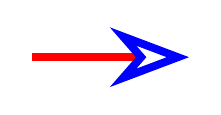
\begin{tikzpicture}
\wall
\draw [red,line width=1mm,-{Stealth[length=1cm,open,blue]}]
(-1,0) -- (1,0);
\end{tikzpicture}


\begin{tikzpicture}
\wall
\draw [red!25,line width=1mm] (-1,0) -- (1,0);
\draw [red,line width=1mm] (-1,-.5) .. controls (0,-.5) and (0,0) .. (1,0);
\end{tikzpicture}

\tikz {
\draw [help lines] (0,-.5) grid [step=1mm] (1,.5);
\draw [thick, red, arrows = {-Stealth[fill=white,length=15pt]}] (0,0) -- (1,0);
}

\tikz \draw [arrows = {-Latex[line width=0.1pt, fill=white, length=10pt]}] (0,0) -- (1,0);

\tikz \draw [arrows = {-Latex[line width=1pt, fill=white, length=10pt]}] (0,0) -- (1,0);

\tikz {
\draw [help lines] (0,-.5) grid [step=1mm] (1,.5);
\draw [thick, red, arrows = {-Stealth[fill=none,length=15pt]}] (0,0) -- (1,0);
}

\tikz {
\draw [help lines] (0,-.5) grid [step=1mm] (1,.5);
\draw [thick, red, arrows = {-Stealth[color=blue, fill=white, length=15pt]}]
(0,0) -- (1,0);
}

\tikz [ultra thick] \draw [draw=red, fill=red!50,
arrows = {-Stealth[length=15pt, fill=pgffillcolor]}]
(0,0) -- (1,1) -- (2,0);

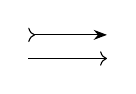
\begin{tikzpicture}
\draw[->] (0,0) -- (1,0);
\draw[>-Stealth] (0,0.3) -- (1,0.3);
\end{tikzpicture}

\begin{tikzpicture}
\draw[-{Stealth[red]}] (0,0) -- (1,0);
\end{tikzpicture}

% Normal case:
\tikz [<->] \draw (0,0) -- (1,0);

\tikz{
\draw [-{Stealth[length=5mm]}] (0,0) -- (2,0);
\draw [|<->|] (1.5,.4) -- node[above=1mm] {5mm} (2,.4);
}

\tikz{
\draw [-{Latex[length=5mm]}] (0,0) -- (2,0);
\draw [|<->|] (1.5,.4) -- node[above=1mm] {5mm} (2,.4);
}

\tikz{
\draw [-{Classical TikZ Rightarrow[length=5mm]}] (0,0) -- (2,0);
\draw [|<->|] (1.5,.6) -- node[above=1mm] {5mm} (2,.6);
}

\tikz \draw [line width=1pt, double distance=3pt,
arrows = {-Latex[length=0pt 3 0]}] (0,0) -- (1,0);

\tikz \draw [line width=1pt, double distance=3pt,
arrows = {-Latex[length=0pt 3 .5]}] (0,0) -- (1,0);

\tikz \draw [line width=1pt, double distance=3pt,
arrows = {-Latex[length=0pt 3 1]} ] (0,0) -- (1,0);

\tikz{
\draw [line width=1mm, -{Stealth[length=10mm, open]}]
(0,0) -- (2,0);
\draw [|<->|] (2,.6) -- node[above=1mm] {10mm} ++(-10mm,0);
}

\tikz{
\draw [line width=1mm, -{Stealth[length=10mm, open, round]}]
(0,0) -- (2,0);
\draw [|<->|] (2,.6) -- node[above=1mm] {10mm} ++(-10mm,0);
}

\tikz \draw [arrows = {-Latex[width=10pt, length=10pt]}] (0,0) -- (1,0);

\tikz \draw [arrows = {-Latex[width=0pt 10, length=10pt]}] (0,0) -- (1,0);

\tikz \draw [arrows = {-Latex[width'=0pt .5, length=10pt]}] (0,0) -- (1,0);

\tikz \draw [arrows = {-Latex[width'=0pt .5, length=15pt]}] (0,0) -- (1,0);

\tikz \draw [arrows = {-Stealth[length=10pt, inset=5pt]}] (0,0) -- (1,0);

\tikz \draw [arrows = {-Stealth[length=10pt, inset=2pt]}] (0,0) -- (1,0);

\tikz \draw [arrows = {-Stealth[inset=0pt, angle=90:10pt]}] (0,0) -- (1,0);

\tikz \draw [arrows = {-Stealth[inset=0pt, angle=30:10pt]}] (0,0) -- (1,0);

\tikz \draw [arrows = {-Stealth[inset=0pt, length=10pt, angle'=90]}]
(0,0) -- (1,0);

\tikz \draw [arrows = {-Stealth[inset=0pt, length=10pt, angle'=30]}]
(0,0) -- (1,0);

\tikz \draw [arrows = {-Stealth[inset=0pt, length=10pt, angle'=90]}]
(0,0) -- (1,0);

\tikz \draw [arrows = {-Stealth[inset=0pt, length=10pt, angle'=30]}]
(0,0) -- (1,0);

\tikz {
\draw [arrows = {-Stealth[]}] (0,1) -- (1,1);
\draw [arrows = {-Stealth[scale length=1.5]}] (0,0.5) -- (1,0.5);
\draw [arrows = {-Stealth[scale length=2]}] (0,0) -- (1,0);
}

\tikz {
\draw [arrows = {-Stealth[]}] (0,1) -- (1,1);
\draw [arrows = {-Stealth[scale width=1.5]}] (0,0.5) -- (1,0.5);
\draw [arrows = {-Stealth[scale width=2]}] (0,0) -- (1,0);
}

\tikz [ultra thick] {
\draw [arrows = {-Hooks[]}] (0,1) -- (1,1);
\draw [arrows = {-Hooks[arc=90]}] (0,0.5) -- (1,0.5);
\draw [arrows = {-Hooks[arc=270]}] (0,0) -- (1,0);
}

\tikz {
\draw [arrows = {->[]}] (0,1) -- (1,1);
\draw [arrows = {->[slant=.5]}] (0,0.5) -- (1,0.5);
\draw [arrows = {->[slant=1]}] (0,0) -- (1,0);
}

% \tikz [>={[slant=.3] To[] To[]}]
% \graph [math nodes] { A -> B <-> C };

\tikz [ultra thick] \draw [arrows = {-Stealth[reversed]}] (0,0) -- (1,0);

\tikz [ultra thick] \draw [arrows = {-Stealth[reversed, reversed]}] (0,0) -- (1,0);

\tikz [ultra thick] \draw [arrows = {-Stealth[harpoon]}] (0,0) -- (1,0);

\tikz [ultra thick] \draw [arrows = {->[harpoon]}] (0,0) -- (1,0);

\tikz [ultra thick] \draw [arrows = {-Stealth[harpoon]}] (0,0) -- (1,0);

\tikz [ultra thick] \draw [arrows = {-Stealth[harpoon,swap]}] (0,0) -- (1,0);

\tikz [line width=2mm]
\draw [arrows = {-Computer Modern Rightarrow[line cap=butt]}]
(0,0) -- (1,0);
\tikz [line width=2mm]
\draw [arrows = {-Computer Modern Rightarrow[line cap=round]}]
(0,0) -- (1,0);
\tikz [line width=2mm]
\draw [arrows = {-Bracket[reversed,line cap=butt]}]
(0,0) -- (1,0);
\tikz [line width=2mm]
\draw [arrows = {-Bracket[reversed,line cap=round]}]
(0,0) -- (1,0);
\end{document}
